\chapter{Topological Spaces}



\section{Random Notes}

\begin{observation}[Some notes on Example 2 page 63]
	In this example we study $ X\subset L^2(-\infty,+\infty) $ the functions in $ L^2(-\infty,+\infty) $ that their primitive functions also belongs to $ L^2(-\infty,+\infty) $. I.e. they roughly look like the following function
	\begin{center}
		\includegraphics[width=0.4\linewidth]{Images/L2WithL2Primitive.png}
	\end{center}
	Then we define the map $ \Phi: X\to X $ given by
	\[ \Phi(x)(t) = \int_{-\infty}^{t} x(\tau) d\tau. \]
	We want to show that this map is not continouse at any point of its domain. Since $ L^2(-\infty,+\infty) $ is a vector space, it is enough to show this for the origin. So we want to show that this map is not continuous at the origin. Let $ x $ be the function whose graph is given as below (the red curve). It is easy to see that the blue curve is its primitive function.
	\begin{center}
	
	\tikzset{every picture/.style={line width=0.75pt}} %set default line width to 0.75pt        
	
	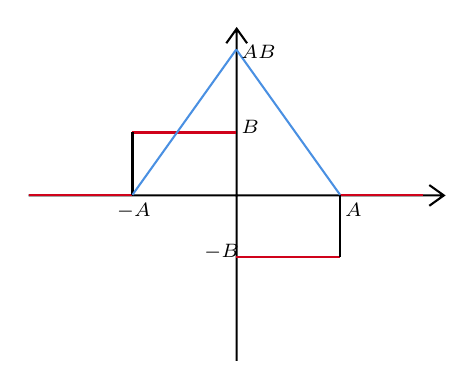
\begin{tikzpicture}[x=0.75pt,y=0.75pt,yscale=-1,xscale=1]
		%uncomment if require: \path (0,300); %set diagram left start at 0, and has height of 300
		
		%Shape: Axis 2D [id:dp36667588747531266] 
		\draw  (130,150.32) -- (330,150.32)(230.2,70) -- (230.2,230) (323,145.32) -- (330,150.32) -- (323,155.32) (225.2,77) -- (230.2,70) -- (235.2,77)  ;
		%Straight Lines [id:da5331057121734024] 
		\draw [color={rgb, 255:red, 208; green, 2; blue, 27 }  ,draw opacity=1 ]   (180,120) -- (230,120) ;
		%Straight Lines [id:da6610509249547099] 
		\draw [color={rgb, 255:red, 208; green, 2; blue, 27 }  ,draw opacity=1 ]   (230,180) -- (280,180) ;
		%Straight Lines [id:da931537369518487] 
		\draw [color={rgb, 255:red, 208; green, 2; blue, 27 }  ,draw opacity=1 ]   (130,150) -- (180,150) ;
		%Straight Lines [id:da8534978395246313] 
		\draw [color={rgb, 255:red, 208; green, 2; blue, 27 }  ,draw opacity=1 ]   (280,150) -- (320,150) ;
		%Straight Lines [id:da730188899085991] 
		\draw    (180,120) -- (180,150) ;
		%Straight Lines [id:da9831547069566817] 
		\draw    (280,150) -- (280,180) ;
		%Straight Lines [id:da4950588238640736] 
		\draw [color={rgb, 255:red, 74; green, 144; blue, 226 }  ,draw opacity=1 ][fill={rgb, 255:red, 74; green, 144; blue, 226 }  ,fill opacity=1 ]   (180,150) -- (230,80) ;
		%Straight Lines [id:da3496559570215123] 
		\draw [color={rgb, 255:red, 74; green, 144; blue, 226 }  ,draw opacity=1 ][fill={rgb, 255:red, 74; green, 144; blue, 226 }  ,fill opacity=1 ]   (230,80) -- (280,150) ;
		
		% Text Node
		\draw (171,152.4) node [anchor=north west][inner sep=0.75pt]  [font=\scriptsize]  {$-A$};
		% Text Node
		\draw (281,152.4) node [anchor=north west][inner sep=0.75pt]  [font=\scriptsize]  {$A$};
		% Text Node
		\draw (231,112.4) node [anchor=north west][inner sep=0.75pt]  [font=\scriptsize]  {$B$};
		% Text Node
		\draw (213,172.4) node [anchor=north west][inner sep=0.75pt]  [font=\scriptsize]  {$-B$};
		% Text Node
		\draw (231,76.4) node [anchor=north west][inner sep=0.75pt]  [font=\scriptsize]  {$AB$};
		
		
	\end{tikzpicture}
\end{center}
		
	 The $ L^2 $ norm is roughly the area under the curve, so the $ L^2 $ norm of $ x $ is $ AB $ while the $ L^2 $ norm of $ \Phi(x) $ is $ AB^2 $. Now to prove that the mapping $ \Phi $ is not continuous at the origin, we need to change $ A,B $ such that the $ L^2 $ norm $ x $ goes to zero but the norm of $ \Phi(x) $ gets larger and larger. Suppose we want to make the norm of $ x $ to be half and double the norm of $ \Phi(x) $. So we need to solve
	\[ \frac{A'B'}{AB} = \frac{1}{2}, \quad \frac{A'B'^2}{AB^2} = 1. \]
	It is easy to see that we need to have
	\[ \frac{A'}{A} = 4, \qquad \frac{B'}{B} = \frac{1}{2}. \]

\end{observation}

\begin{observation}[Some notes on Example 4, page 64]
	Putting this example in contrast to the example above, teaches us a lot! In the example above we observed that the ``integration'' of $ L^(-\infty,+\infty) $ functions is nowhere continuous. However, in this example, we will see that the integration operator in $ L^2[0,T] $ is a uniformly  continuous operator! This is a huge contrast and the surprising fact is that in both cases we are dealing with the ``same'' operator and the only difference is their domain. To see this let $ X = L^2[0,T] $ and let $ \Phi: L^2[0,T] \to L^2[0,T] $ defined as
	\[ [\Phi(x)](t) = \int_{0}^{t} x(\tau)d\tau. \]
	\begin{remark}
		We need to check to see if $ \Phi(x) $ really belongs to $ L^2[0,T] $. However the argument will be very similar to what we will see below, so we have skipped this part. 
	\end{remark}
	Since $ L^2[0,T] $ is a vector space and $ \Phi  $ is a linear map, it is enough to show the continuity at the origin. Let $ x\in L^2[0,T] $. Then
	\begin{align*}
		d(\Phi(x),0)^2 &= \int_{0}^{T} \abs{\int_{0}^{t} [\Phi(x)](\tau)d\tau}^2 dt \leq \int_{0}^{T} \left(\int_{0}^{t} \abs{[\Phi(x)](\tau)}d\tau\right)^2 dt \\ 
		& \leq \int_{0}^{T} \left(\int_{0}^{T} \abs{[\Phi(x)](\tau)}d\tau\right)^2 dt \\
		& \leq \int_{0}^{T} \left( \int_{0}^{T} 1 d\tau \right) \left( \int_{0}^{T}\abs{[\Phi(x)](t)}^2 d\tau \right) dt \\
		&= T^2 \int_{0}^{T}\abs{[\Phi(x)](t)}^2 d\tau \\
		&= T^2 d(x,0).
	\end{align*}
	So we have
	\[ d(\Phi(x),0) \leq T d(x,0). \]
	Since the expansion factor $ T $ does not depend on $ x $, we can conclude that $ \Phi $ is actually uniformly continuous.
\end{observation}

\begin{observation}[Discrete version of the example above]
	We can construct a discrete version of the example above, where the underlying space is $ \R^n $, and the integration operator $ \Phi $ is a linear map $ \Phi: \R^n \to \R^n $ given by
	\[ \Phi: \begin{bmatrix}
		x_1 \\ x_2 \\ x_3 \\ \vdots \\ x_n
	\end{bmatrix} \mapsto 
	\begin{bmatrix}
		x_1 \\ x_1+x_2 \\ x_1+x_2+x_3 \\ \vdots \\ x_1+\cdots+x_n
	\end{bmatrix}.
	 \]
	 This can be represented by the matrix
	 \[ M = \begin{bmatrix}
	 	1 & 0 & 0 & 0 & \cdots & 0 \\
	 	1 & 1 & 0 & 0 & \cdots & 0 \\
	 	1 & 1 & 1 & 0 & \cdots & 0 \\
	 	1 & 1 & 1 & 1 & \cdots & 0 \\
	 	\vdots & \vdots & \vdots & \vdots & \ddots & \vdots  \\
	 	1 & 1 & 1 & 1 & \cdots & 1
	 \end{bmatrix} \]
	 However, from the Example 1 from page 62 we know that a linear map between vector spaces is continuous with the operator norm at most $ \sum_{ij} \abs{m_{i,j}} $. So the operator norm of this matrix will be
	 \[ \norm{\Phi} \leq  \left( \frac{n(n+1)}{2} \right)^{1/2} \approx n. \]
\end{observation}

\begin{summary}[Some notes on Example 5 on page 65]
	The example 5 demonstrates the observation above in a very useful way. It explicitly shows that the example above is just a very special matrix and we can have more general linear maps with arbitrary elements in their matrix representation. So the matrix operators between finite dimensional vector spaces correspond to the integration kernels. consider $ L_2[0,T] $ and let $ k \in L^2([0,T]\times [0,T]) $, i.e.
	\[ \int_{0}^{T} \int_{0}^{T} \abs{k(t,\tau)}^2 d\tau dt = M^2 < \infty. \] 
	And we define the linear map $ \Phi_k: L_2[0,T] \mapsto L_2[0,T] $ 
	\[ [\Phi_k(x)](t) = \int_{0}^{T} k(t,\tau)  x(\tau) d\tau.  \]
	The Example 5 shows that this is a continouse map (bounded linear map) with operator norm 
	\[ \norm{\Phi_k} \leq M. \]
	Compare this with Example 1.
	
	\begin{remark}
		One special kind of kernel integrals are convolutions where the kernel is of the form $ k(t,\tau) = h(t-\tau) $ for some function $ h $ of appropriate type (I think it is enough to have $ L_2[0,T] $, with the definition that $ h(t-\tau) = 0 $ if $ t-\tau \notin [0,T] $). We often write convolution as
		\[ (f\ast h) (t) = \int_{0}^{t} h(t-\tau)f(\tau) d\tau. \]
	\end{remark}
\end{summary}



\section{Solved Problems}


\subsection{Metric Spaces}

\begin{summary}[A metric for bounded functions defined on any set $ S $]
	Let $ S $ be a nonempty set and let $ X = B(S) $ denote the collection of all bounded real-valued functions defined on $ S $. Then
	\[ d(f,g) = \sup\set{\abs{f(s)-g(s)}:s\in S}, \]
	is a metric on $ X $.
\end{summary}

\begin{summary}[A metric for differential operators]
	Let $ X(n) $ denote all the differential operators of the form
	\[ P(D) = p_0D_0 + p_1D_1 + \cdots + p_nD_n. \]
	Then $ d $ is a metric on $ X(n) $:
	$ d(P(D),Q(D)) = \sum_{i=0}^{n} \abs{p_i - q_i} $.
\end{summary}


\begin{summary}
	Let $ X $ denote the collection of all bounded closed intervals $ [a,b] $ from the real line. Let $ [a,b] $ and $ [c,d] $ be two sets. Then the symmetric difference $ [a,b] \delta [c,d] $ is the union of at most two bounded intervals. $ \rho([a,b],[c,d]) $ to be the sum of the lengths of these intervals. Then $ \rho $ is a pseudometric. In particular, the distance between any two single points is zero.
\end{summary}
\begin{remark}
	{\color{red} \noindent TODO:} I am still thinking why the triangle inequality of the metric defined above holds.
\end{remark}

\begin{problem}
	Let $ d $ be a metric on $ X $ and let $ d_\alpha = \alpha d $, where $ 0 < \alpha < 1 $. Show that $ d_\alpha \not\equiv d $ if $ X $ has more than two points.
\end{problem}
\begin{solution}
	Let $ X $ have more than one point. Then $ \exists x,y \in X $ such that $ d(x,y) \neq 0 $. Then $ d(x,y) \neq \alpha d(x,y) = d_\alpha(x,y) $. So $ d \not\equiv d_\alpha $.
\end{solution}


\begin{problem}
	Show that $ d(x,y) = \abs{x-y} $ is a metric on the real number $ \R $. Show that it is also a metric on the set of complex numbers $ \C $.
\end{problem}

\begin{solution}
	First, we show $ (\R, d) $ is a metric space. We need to show:
	\begin{enumerate}[(i)]
		\item First, we show that $ d $ is always positive. Since $ \abs{x} = \max\set{x,-x} $, we have $ \pm x \leq \abs{x} $. Adding to two inequalities we will get $ 0\leq \abs{x} $. Now we want to show that $ \abs{x-y}=0 $ then $ x = y $. $ \abs{x-y} = 0 $ implies $ x-y= 0 $, and then we will have $ x=y $.
 		\item Since $ \abs{x-y} = \max{x-y,y-x} $, we will have $ \abs{y-x} = \max{y-x,x-y} = \abs{x-y} $.
		\item Triangle inequality: From the definition of absolute value we have $ \abs{x} = \max\set{x,-x} $. So $ x\leq \abs{x} $ and $ -\abs{x} \leq x $. Let $ a,b \in \R $. Then 
		\[ a\leq \abs{a},\ b\leq \abs{b} \quad\implies\quad  a+b \leq \abs{a} + \abs{b}. \]
		Furthermore, 
		\[ -\abs{a}\leq a,\ -\abs{b}\leq b \quad\implies\quad -\abs{a}-\abs{b} \leq a+b.   \]
		Combining these two inequalities, we will get
		\[ -\abs{a} - \abs{b} \leq a+b \leq \abs{a} + \abs{b}. \]
		So
		\[ \abs{a+b} \leq \abs{a} + \abs{b}. \]
		
		Now we show that $ (\C,d)$ is a metric space. For this purpose we can utilize the properties of the complex conjugation and work with the definition  $ \abs{z_1-z_2} = \sqrt{(z_1-z_2)\conj{(z_1-z_2)}} $. But instead, we want to show that there is a bijection from $ (\C,d) $ (we don't know yet if it is a metric space, otherwise we could call this map an isometric bijection) to $ (\R^2,d_{\R^2}) $. Recall
		\[ \C = \set{a+ib:\ a,b\in \R}. \]
		Let $ \phi: \C\to\R^2 $ given by $ a+ib \mapsto (a,b) $. This is a bijection, since for any $ a+ib\in \C $ we have a unique $ (a,b)\in\R^2 $ (uniquely determined by $ a,b $), and for any $ (a,b)\in \R^2 $ we have a uniquely determined $ a+ib\in \C $. Also we claim that
		\[ d(z,w)  = d_{\R^2}(\phi(z),\phi(w)). \]
		This is true because
		\[ d(z,w) = d(z_1+iz_2, w_1+iw_2) = \sqrt{(z_1-w_1)^2+(z_2-w_2)^2} = d_{\R^2}((z_1,z_2),(w_1,w_2)) = d_{\R^2}(\phi(z),\phi(w)). \]
		We can use this map to transfer all of the properties of $ d_{\R^2}  $ in $ \R^2 $ to $ d $ in $ \C $. So $ (\C,d) $ is indeed a metric space. So now we can call $ \phi $ an isometric bijection.
	\end{enumerate}
\end{solution}

\begin{remark}
	In the question above, for $ (\R,d) $ we used the definition $ \abs{x} = \max\set{x,-x} $, and for $ (\C,d) $ we used the definition $ \abs{x} = \sqrt{x\conj{x}}. $
\end{remark}


\begin{problem}
	Let $ d(x,y) $ be a metric on $ X $. Show that 
	\[ d_1(x,y) = \frac{d(x,y)}{1+d(x,y)}, \qquad d_2(x,y) = \min\set{1,d(x,y)}, \]
	are also metrics on $ X $. Show that every set in the metric space $ (X,d_1) $ and $ (X,d_2) $ is bounded.
\end{problem}
\begin{solution}
	\begin{enumerate}[(i)]
		\item Showing that $ d_1(x,y) $ is a metric: Positive definiteness: since the enumerator and denumenator are both positive, then $ d_1(x,y) $ is also positive for all $ x,y\in X $. Let $ x,y\in X $ such that $ d_1(x,y) =0 $. This implies $ d(x,y) =0 $, hence $ x=y $. Symmetry follows from $ d $ being symmetric. For the triangle inequality we use the fact that $ f(x) = \frac{x}{1+x} $ is strictly increasing for $ x\geq 0 $ (because it has positive derivative), and also it is subadditive. To see the subadditivity, observe that
		\[ f(x+y) \leq \frac{x+y}{1+x+y} = \frac{x}{1+x+y} + \frac{y}{1+x+y} \leq \frac{x}{1+x} + \frac{y}{1+y} = f(x) + f(y).  \]
		Using the fact that for all $ x,y,z\in X $ we have
		\[ d(x,z) \leq d(x,y) + d(y,z), \]
		using the monotinicity of $ f $ and then its sub additivity, we will get
		\[ d_2(x,z) \leq d_2(x,y) + d_2(y,z). \]
		(See the summary box below for a detailed argument of a more general setting).
		
		\item Showing that $ d_2(x,y) = d(x,y)\wedge 1 $ is a metric: Positive definiteness: Since $ d(x,y) \geq 0 $ then $ d(x,y)\wedge 1 \geq 0 $. Let $ x,y \in X $ such that $ d(x,y) \wedge 1 = 0 $. So $ d(x,y) = 0 $. This implies $ x=y $. So $ d_2 $ is positive definite. Symmetric: Let $ x,y\in X $. Then $ d_2(x,y) = d(x,y)\wedge 1 = d(y,x)\wedge 1 = d_2(y,x) $, where we have used the fact that $ d(x,y) = d(y,x) $. So $ d_2(x,y) = d_2(y,x) $. For the triangle inequality we use the following lemma:
		\begin{lemma}
			Let $ a,b \geq 0 $. Then 
			\[ a < b \qquad \implies \quad a\wedge 1 \leq b \wedge 1. \]
			Also
			\[ (a+b) \wedge 1 \leq a\wedge 1 + b\wedge 1. \]
			
			\begin{proof}
				For the first implication, when $ a<b $, then there are three cases: $ 0\leq a < b \leq 1,\ 0\leq a \leq 1 < b, 1 < a<b $. In the first case $ a\wedge 1 = a, b\wedge 1 = b $ So $ a\wedge 1 \leq b\wedge 1 $ holds. This holds for the other cases as well.
				
				For the second implication, again we will show in cases: When $ a+b < 1,\ a+b = 1,\ a+b>1 $. For the first case we can only have $ a,b < 1 $. So $ (a+b)\wedge 1= a+b,\ a\wedge 1 = a,\ b\wedge 1 = b $. So the desired inequality holds. For the second case, again $ a=a\wedge 1,\ b=b\wedge 1 $, and $ (a+b)\wedge 1 = a+b =1 $. So the desired inequality holds. For the third case, WLOG we can assume that $ a\leq b $. Since $ a+b \geq 1 $, then at least one of $ a $ or $ b $ should be larger than 1. WLOG we can assume $ a\geq 1 $. So $ (a+b)\wedge 1 = 1 $ and $ a\wedge 1 = 1 $. So the desired inequality holds.
			\end{proof}
		\end{lemma}
		So by the triangle inequality $ d(x,z)\leq d(x,y) + d(y,z) $, and using the lemma above we can conclude that
		\[ d(x,z) \wedge 1 \leq d(x,y)\wedge 1 + d(y,z) \wedge 1. \]
	\end{enumerate}
	
	Now to show that all of the sets in $ X $, with the metrics above are bounded, it is enough to observe that for all $ x,y \in X $ we have $ d_1(x,y) \leq 1 $ and $ d_2(x,y) \leq 1 $.
\end{solution}
\begin{summary}[Transformation of the metric]
	Using the proof ideas of the examples above, we can generalize it in the following proposition.
	\begin{proposition}
		Let $ (X,d) $ be a metric space and $ \phi:[0,+\infty)\to \R $ be a real valued functions such that
		\begin{enumerate}[(i)]
			\item $ \phi(x) = 0 $ if and only if $ x = 0 $.
			\item monotone increasing,
			\item subadditive: $ \forall x,y \geq 0 $ we have $ \phi(x+y) \leq \phi(x) + \phi(y) $.
			Then $ \tilde{d} = \phi\circ d $ is also a metric, and $ (X,\tilde{d}) $ is a metric space.
		\end{enumerate}
	\end{proposition}
	\begin{proof}
		Since $ \phi(x) = 0 $ if and only if $ x = 0 $, then $ \tilde{d} = 0 $ if and only if $ d = 0 $, if and only if $ x=y $. So $ \tilde{d} $ is positive definite. $ \tilde{d} $ is also symmetric, because $ \forall x,y \in X $, we have $ d(x,y) = d(y,x) $ that implies $ \tilde{d}(x,y) = \phi(d(x,y)) = \phi(d(y,x)) = \tilde{d}(y,x). $ For the triangle inequality, we have
		\[ d(x,z) \leq d(x,y)  + d(y,z). \]
		We apply (ii) above and we will get
		\[ \tilde{d}(x,z) \leq \phi(d(x,y) + d(y,z)), \]
		and we now apply (iii) above to get
		\[ \tilde{d}(x,z) \leq \tilde{d}(x,y) + \tilde{d}(y,z). \]
	\end{proof}
\end{summary}


\begin{summary}[Metric transformation examples]
	Using the example above, and the remark below, the followings are example functions that can transform a metric $ d $ to a new metric $ \tilde{d} = f(d) $.
	\begin{enumerate}[(i)]
		\item $ f_1(x) = x\wedge 1 $.
		\item $ f_2(x) = x/(1+x) $.
		\item $ f_3(x) = x^\alpha/(1+x^\alpha) $ for $ 0<\alpha\leq1 $.
	\end{enumerate}
	\begin{remark}
		The reason that the example (iii) above works is that $ f_3 $ satisfies all the properties in the summary box above. To see the sub-additivity, it is enough to show the sub-additivity of $ x^\alpha $ when $ 0 < \alpha \leq 1 $. Let $ \alpha = 1-\beta $. Then 
		\[ (x+y)^\alpha = \frac{x+y}{(x+y)^\beta} < \frac{x}{(x+y)^\beta} + \frac{y}{(x+y)^\beta} \leq \frac{x}{x^\beta} + \frac{y}{y^\beta} = x^\alpha + y^\alpha.z  \]
	\end{remark}
\end{summary}


\begin{problem}
	A real-valued function $ \rho(x,y) $ is said to be a pseudometric on $ X $ if it satisfies conditions (M1), (M3), and (M4).
	\begin{enumerate}[(a)]
		\item Show that $ \rho(x,y)\equiv 0 $ is a pseudometric on any set $ X $.
		\item Show that $ \rho((x_1,x_2),(y_1,y_2)) = \abs{x_1-y_1} $ is a pseudometric in the plane $ \R^2 $.
	\end{enumerate}
\end{problem}
\begin{solution}
	\begin{enumerate}[(a)]
		\item $ \rho(x,y)\equiv 0 $ satisfies $ (M1), (M3) $, and $ (M4) $ vacuously. However, if $ X $ has only one element, then $ \rho $ is indeed a metric. But if $ X $ has more than two elements, then $ \exists x,y \in X $ such that $ x\neq y $ but $ \rho(x,y) = 0 $.
		
		\item Being symmetric (M3) and the triangle inequality (M4) follows from the properties of $ \abs{\cdot} $. However, for all $ x,y \in \R^2 $ that have the same first component (i.e. points on the vertical lines) have $ d(x,y) = 0 $. However, this will be a metric on the quotient space $ \R^2/W $ where $ W = \operatorname{Span}\set{(0,1)} $.
  	\end{enumerate}
\end{solution}

\begin{problem}
	Show that if $ A $ is nonempty, in a metric space $ (X,d) $, then $ \operatorname{diam}A = 0 $ if and only if $ A $ consist of a single point. Is this true in a pseudometric space?
\end{problem}
\begin{solution}
	For the forward direction assume for $ A\subset X $ we have $ \operatorname{diam}A = 0 $. So
	\[ \sup_{x,y \in A} \set{d(x,y)} = 0. \]
	This implies that $ \forall x,y \in A $ we have $ d(x,y) = 0 $. Since $ d $ is a metric, then $ A = \set{x} $ is a singleton. For the converse, let $ A = \set{x} $. Then it follows immediately that $ \operatorname{diam} A  = 0 $.
	
	No this is not true in the case of the pseudometric spaces. In our proof above, in the forward direction, the logic breaks if $ d $ is a pseudometric. I.e. it is possible to have $ \sup_{x,y\in A}\set{d(x,y)} = 0 $ but $ A $ is not singleton.
\end{solution}


\subsection{Examples of Metric Spaces}

\begin{problem}
	Let $ X=\R^2 $ and let 
	\[ d(x,y) = (\abs{x_1-y_1}^{1/2} + \abs{x_2-y_2}^{1/2})^2. \]
	Is $ (X,d) $ a metric space?
\end{problem}
\begin{solution}
	No. Because the triangle inequality breaks. Let 
	\[ x = (0,0), \qquad y = (0,1/4), \qquad z = (1/4,1/4). \]
	It is easy to check that the triangle inequality $ d(x,z) \leq d(x,y) + d(y,z) $ does not hold. Because
	\[ 1 = d(x,z) \leq d(x,y) + d(y,z) = 1/4 + 1/4 = 1/2, \]
	is a contradiction.
	\begin{remark}
		With a similar idea of proof, it is easy to show that $ d_p $ fails to satisfy the triangle inequality if $ 0<p<1 $.
	\end{remark}
\end{solution}

\begin{problem}
	In $ \R^2 $ let $ A \set{x=(x_1,x_2): (\abs{x_1}^2 + \abs{x_2}^2)^{1/2} < 1} $, and
	\[ d(x,y) = \set{\abs{x_1-y_1}^2 + \abs{x_2-y_2}^2}^{1/2}. \]
	Compute $ d(x,A) $. Show that $ d(x,A) = 0 $ if and only if 
	\[ \abs{x_1}^2 + \abs{x_2}^2 \leq 1. \]
\end{problem}
\begin{solution}
	Let $ x = (x_1,x_2) \in \R^2 $ (WLOG we assume that $ x_1>0 $) that does not belong to $ A $. The ray that passes through $ x $ is given by $ y = \frac{x_2}{x_1}x $, and this ray intersects the unit circle at
	\[ \tilde{x} = (\frac{1}{\sqrt{1+(x_2/x_1)^2}}, \frac{x_2/x_1}{\sqrt{1+(x_2/x_1)^2}} ). \]
	So the distance between $ x $ and the point above is
	\[ d(x,\tilde{x}) = \left( \abs{\frac{1}{\sqrt{1+(x_2/x_1)^2}}-x_1}^2 + \abs{\frac{x_2/x_1}{\sqrt{1+(x_2/x_1)^2}}-x_2}^2 \right)^{1/2}. \]
	
	To show that $ d(x,A) = 0 $ if and only if $ x_1^2 + x_2^2 \leq 1 $, we first do the forward direction. Let $ d(x,A) = 0 $. From our explicit formula above, it is easy to see that we should have
	\[ x_1 = \frac{1}{\sqrt{1+(x_2/x_1)^2}}, \qquad x_2 = \frac{x_2/x_1}{\sqrt{1+(x_2/x_1)^2}}.  \]
	It is easy to check that $ x_1^2 + x_2^2 =1 $ which implies $ x_1^2 + x_2^2 \leq 1 $. For the converse direction, we assume $ x_1^2 + x_2^2 \leq 1 $. When $ x_1^2 + x_2^2 < 1 $, then $ x\in A $, and by the definition of $ d(x,A) $ we see $ d(x,A) = 0 $. When $ x_1^2 + x_2^2 = 1 $, then we can write $ 1+(x_1/x_2)^2 = 1/x_1^2 $. Using the fact that $ x_1 > 0 $ this implies that
	\[ d(x,A) = 0, \]
	where we have used the explicit formula above.
\end{solution}


\begin{problem}
	In example 5, the metric $ d_\infty $ was defined with a ``sup'' instead of ``max''. In order to see the necessity of this let $ x = (x_1,x_2,\cdots), y = (y_1,y_2,\cdots) $ be given by 
	\[ x_n = \frac{1}{n+1}, \qquad  y_n = \frac{n}{n+1}. \]
	And argue why ``sup'' should be used instead of ``max''? What about Example 8 and Example 11?
\end{problem}
\begin{solution}
	The reason is that if on $ \ell_\infty $ we define $ d_\infty $ by ``max'', then for the presented examples $ d_\infty(x,y) $ does not exist. In the case of example 8, we \textbf{can} replace ``max'' with ``sup''. The reason is that if $ x,y \in C[0,T] $, then $ f = \abs{x-y} \in C[0,T] $. On the other hand, a continuous function defined on a compact set, attains its maximum and minimum. For Example 11, we can \textbf{not} use ``max'' in place of ``sup''.
\end{solution}


\begin{problem}
	Sketch the set of points $ x=(x_1,x_2) $ in $ \R^2 $ for which 
	\[ d_p(0,x) = 1, \]
	where $ 0=(0,0) $ and $ d_p $ is defined in Example 1. With $ x,y $ fixed show that $ d_p(x,y) $ is decreasing in $ p $. Hence
	\[ d_p(x,y) \leq d_q(x,y). \]
\end{problem}
\begin{solution}
	It is easy to find such sketches online. For the second part, fix $ x,y\in \R^2 $. Then
	\[ \frac{d d_p(x,y)}{dp} = -\frac{A}{p^2}, \]
	where $ A $ is a positive quantity (can be calculated explicitly by using the chain rule). So $ d_p(x,y) $ is decreasing.
\end{solution}
\begin{summary}
	For fixed $ x,y\in \R^n $, $ d_p(x,y) $ is decreasing in $ p $. So 
	\[ p\leq q \quad \implies \quad d_p(x,y) \geq d_q(x,y). \]
\end{summary}

\begin{problem}
	Let $ C $ be the unit circle in the complex plane, that is $ C = \set{z:\abs{z}=1} $. Let $ X $ denote all complex-valued functions $ f(z) $ defined on $ C $ for which
	\[ \int_C \abs{f(z)}dz < \infty. \]
	Show that 
	\[ d(f,g) = \left(\int_C \abs{f(z)-g(z)}dz\right)^{1/2} = \left(\int_{0}^{2\pi} \abs{f(e^{2i\pi\theta}) - g(e^{2i\pi\theta})}d\theta \right)^{1/2}  \]
	is a metric on $ X $.
\end{problem}
\begin{solution}
	It is easy to check the other properties of being a metric. Thus we will show that $ d $ satisfies the triangle inequality. To see this let $ f,g,h \in X $. Then 
	\begin{align*}
		d(f,g) = \left( \int \abs{\tilde{f} - \tilde{g}}^2  \right)^{1/2} = \left( \int \abs{\tilde{f} -\tilde{g} \pm \tilde{h}}^2 \right)^{1/2} = \left( \int \abs{u+v}^2  \right)^{1/2},
	\end{align*}
	where $ u = \tilde f - \tilde h $ and $ v = \tilde{h} - \tilde{g} $, and $ \tilde{f}(\theta) = f(e^{2i\pi\theta}) $. Observe that
	\[ \int \abs{u+v}^2 = \int (u+v) \conj{(u+v)} = \int (\abs{u}^2 + \abs{v}^2 + 2\Re{u\conj{v}}) = \int \abs{u}^2 + \int \abs{v}^2 + 2\int \Re{u\conj{v}}.\]
	Also
	\[ \int \Re{u\conj{v}} \leq \Re{ \int u\conj{v}} \leq \Re{\norm{u}\norm{v}} = \norm{u}\norm{v},  \]
	where $ \norm{\cdot} $ is the norm that induces the metric. So
	\[ \int \abs{u+v}^2 \leq \norm{u}^2 + \norm{v}^2 + 2\norm{u}\norm{v} = (\norm{u} + \norm{v})^2. \]
	so we can conclude
	\[ d(f,g) = \left( \int \abs{u+v}^2 \right)^{1/2} \leq \norm{u} + \norm{v} = d(f,h) + d(h,g). \]
\end{solution}

\begin{problem}
	Let $ X $ denote the class of all complex-valued functions $ f(z) $ that are analytic for $ \abs{z} < 1 $. Let $ f(z) = \sum_{n=0}^{\infty} a_nz^n $ and $ g(z) = \sum_{n=0}^{\infty} b_n z^n $ be the power series expansion for $ f,g $ in $ X $. Show that the following functions are metrics, or pseudo-metrics.
	\begin{enumerate}[(a)]
		\item $ d(f,g) = \sup\set{\abs{f(z)-g(z)}\ :\ \abs{z}\leq \rho} $, where $ 0 < \rho < 1 $.
		\item $ d(f,g) = \abs{a_0 - b_0} $.
		\item $ d(f,g) = \abs{a_0 - b_0} + \abs{a_1 - b_1} $.
		\item $ d(f,g) = \sum_{n=0}^{\infty} \abs{a_n - b_n}\rho^n $, where $ 0<\rho<1 $.
		\item 
		\[ d(f,g) = \sup\set{\abs{\int_{\abs{\xi}=0} \frac{f(\xi) - g(\xi)}{z-\xi}d\xi}\ :\ \abs{z} < \rho}, \quad \text{where $ 0<\rho<1 $.} \]
	\end{enumerate}
\end{problem}

\begin{solution}
	Since we need to choose between a metric or a pseudometric, we don't check the triangle inequality.
	\begin{enumerate}[(a)]
		\item Is a metric. 
		\item Is a pseudometric. Because the distance between functions in which in their expansion only the first term is the same will be zero.
		\item Is a pseudometric. Because of a similar argument as above.
		\item Is a metric. Because if $ d(f,g) = 0 $, then every term in the positive series should be zero, hence $ \abs{a_n - b_n} = 0 $ for all $ n\in \N $.
		\item {\color{red} \noindent Still thinking!}
	\end{enumerate}
\end{solution}



\subsection{Continuity}


\begin{problem}
	Let $ C^\infty[0,T] $ denote the set of all real-valued smooth functions defined on $ [0,T] $. Let $ D $ be the mapping of $ C^\infty[0,T] $ to itself defined by
	\[ Df = \frac{df}{dt}. \]
	\begin{enumerate}[(a)]
		\item Let $ d_1 $ be the sup-metric on $ C^\infty[0,T] $. Is $ D $ a continuous mapping  of $ (C^\infty[0,T],d_1) $ into itself?
		
		\item Define a metric $ d_2 $ on $ C^\infty[0,T] $ by
		\[ d_2(x,y) = d_1(x,y) + d_1(Dx,Dy). \]
		Is $ D $ a continouse mapping of $ (C^\infty[0,T], d_2) $ into $ (C^\infty[0,T], d_1) $?
	\end{enumerate}
\end{problem}
\begin{solution}
	\begin{enumerate}[(a)]
		\item No. Consider the sequence of functions $ (f_n)_n $ where 
		\[ f_n(t) = \frac{\sin(2^n x)}{n}. \]
		Then $ d_1(f_n, 0)\to 0 $ as $ n\to \infty $ but $ d_1(Df_n, 0) $ becomes arbitrary large. 
		
		\item Yes. Let $ f,g \in  C^\infty[0,T] $ then
		\[ d_1(Df, Dg) \leq d_1(Df, Dg) + d_1(f,g) = d_2(f,g). \]
		So for any $ \epsilon>0 $ we let $ \delta = \epsilon $. Then if $ d_2(f,g) < \delta $ it implies that $ d_1(f,g) < \epsilon $.
	\end{enumerate}
\end{solution}

\begin{problem}
	A delay line is a device whose output is ideally a delayed version of its input, i.e.
	\[ y(t) = x(t-\tau). \]
	Suppose that $ x,y \in L_2(-\infty,+\infty) $, where $ L_2(-\infty,+\infty) $ has the usual metric. Is the mathematical model of the delay line a continouse mapping of $ L_2(-\infty,+\infty) $ into itself?
\end{problem}

\begin{solution}
	We know that integration, in the sense of Lebesgue, is not sensitive to shift. I.e.
	\[ \int_{-\infty}^{+\infty} f(t) dt = \int_{-\infty}^{+\infty} f(t-\tau) dt, \]
	for all $ \tau \in \R $. So for any $ f,g \in L_2(-\infty,+\infty) $ we have
	\[ d(f,g) = d(Sf, Sg). \]
\end{solution}



\begin{problem}
	Let $ Y = C[0,T] $ be given with the sup-metric $ d(x,y) $. Let 
	\[ X = (C[0,T],d) \times (C[0,T],d), \]
	be the product space. Consider the mapping $ F $ of $ X $ into $ Y $ defined by $ F(x) = x_1x_2 $, where $ x=(x_1,x_2) $. (That is $ F $ is a multiplier). Is $ F $ continuous? Is $ F $ uniformly continuous?
\end{problem}
\begin{solution}
	Assume that the norm on $ X $ is $ d_2(f,g) = d(f_1,g_1) + d(f_2,g_2) $ (we could chose other metrics on the product space as well, but we chose this one for the convenience). Then we can write
	\begin{align*}
		d(F(f),F(g)) &= \sup_{t\in[0,T]} \abs{[F(f)](t) - [F(g)](t)} \\
		&= \sup_{t\in[0,T]} \abs{f_1(t)g_1(t) - f_2(t)g_2(t)} \\
		&= \sup_{t\in[0,T]} \abs{f_1(t)g_1(t) - f_2(t)g_2(t) \pm f_1(t)g_2(t)} \\
		&= \sup_{t\in[0,T]} \abs{f_1(t)(g_1(t)-g_2(t)) + g_2(t)(f_1(t)-f_2(t))} \\
		&\leq \norm{f_1}_\infty d(g_1,g_2) + \norm{g_2}_\infty d(f_1,f_2) \\ 
		&\leq \max\set{\norm{f_1}_\infty, \norm{g_2}_\infty} (d(g_1,g_2)+d(f_1,f_2)) \\
		&= \max\set{\norm{f_1}_\infty, \norm{g_2}_\infty} d_2(f,g).
	\end{align*}
	So for a given $ \epsilon>0 $ we can let $ \delta = \epsilon/(\max\set{\norm{f_1}_\infty, \norm{g_2}_\infty}) $. However, since the choice of $ \delta $ depends on the point $ f,g $, then the uniform continuity fails.
\end{solution}


\begin{problem}
	Let $ (X,d) $ be a metric space, where $ X $ is nonempty. Let $ Y = BC(X,\R) $ denote the collection of all bounded, continuous real-valued functions defined on $ X $. 
	\begin{enumerate}[(a)]
		\item Show that the functions
		\begin{align*}
			f_1 &: x\mapsto \frac{d(x,x_0)}{1+d(x,x_0)}, \\
			f_2 &: x\mapsto d(x,x_1) - d(x,x_0), \\
			f_3 &: x\mapsto 3,
		\end{align*}
		are in $ Y $.
		
		\item Show that 
		\[ \sigma(f,g) = \sup\set{\abs{f(x)-g(x)}: x\in X} \]
		is a metric on $ Y $.
	\end{enumerate}
\end{problem}

\begin{solution}
	\begin{enumerate}[(a)]
		\item Fix $ x_0\in X $. We want to show the function $ f:X\mapsto \R $ given as $ f(x) = d(x,x_0) $ is a continuous function. Because
		\[ d(f(x),f(y)) = \abs{f(x)-f(y)} = \abs{d(x,x_0)+d(y,y_0)} \leq \abs{d(x,y)+d(y,x_0)-d(y,x_0)} = d(x,y). \] 
		On the other hand since the function $ g:\R\to\R $ given by $ x\mapsto x/(1+x) $ is a bounded continouse function, then $f_1 =  d/1+d $ is also a bounded continouse function. Continuoity of $ f_2 $ follows from a similar reasoning. For the boundedness, observe that 
		\[ d(x,x_1) - d(x,x_0) \leq d(x,x_0) + d(x_0,x_1) - d(x,x_0) = d(x_0,x_1). \]
		
		\item Follows from the result of Exercise 13 page 56.
	\end{enumerate}
\end{solution}


\begin{problem}
	Let $ f: X \to X $ be a continuous mapping, where $ X $ has a metric $ d $. Let $ G(f) $ denote the graph of $ f $ in $ X\times X $, and $ \Delta $ the diagonal set
	\[ \Delta = \set{(x,y): x=y} = \set{(x,x):x\in X}. \]
	Assume that $ X\times X $ has the metric 
	\[ d((x_1,y_1),(x_2,y_2)) = d(x_1,x_2) + d(y_1,y_2). \]
	Define $ g: \Delta \to G(f) $ by
	\[ g(x,x) = (x,f(x)). \]
	Show that $ g $ is continuous. Show that $ g $ is invertible. Is $ \inv{g} $ continuous?
\end{problem}

\begin{solution}
	$ g $ is continuous. To see this let $ (x_1,x_1), (x_2,x_2) \in \Delta $. So
	\begin{align*}
		d(g(x_1,x_1), g(x_2,x_2)) &= d((x_1,f(x_1)), (x_2,f(x_2))) \\
		&= d(x_1,x_2) + d(f(x_1),f(x_2)) \\
		&\leq (1+A(x_1,x_2))d(x_1,x_2) \\
		&= \frac{1}{2}(1+A(x_1,x_2))d((x_1,x_1), (x_2,x_2)).
	\end{align*}
	where we have used the continuity of $ f $, i.e. $ d(f(x_1),f(x_2)) \leq A(x_1,x_2) d(x_1,x_2) $.
	So $ g $ is a continuous mapping. Define the inverse of $ g $ as
	\[ h= \inv{g}: G(f)\to \Delta, \qquad \inv{g}(x,f(x)) = (x,x). \]
	$ \inv{g} $ is indeed inverse of $ g $ as it is straightforward to check $ \inv{g}\circ g $ and $ g\circ\inv{g} $ are both identity maps. However, $ h = \inv{g} $ is not necessarily continuous. To see this let $ (x_1,f(x_1)), (x_2,f(x_2)) \in G(x) $. Then
	\[ d(h(x_1,f(x_1)), h(x_2,f(x_2))) = d((x_1,x_1),(x_2,x_2)) = d(x_1,x_2) + d(x_1,x_2) = 2d(x_1,x_2). \]
	So we can come up with examples where $ (x_1,x_1) $ and $ (x_2,x_2) $ are close to each other, but $ (x_1,g(x_1)) $ and $ (x_2,g(x_2)) $ are not. For instance consider the following graph:
	\begin{figure}[h!]
	\centering
	
	
	\tikzset{every picture/.style={line width=0.75pt}} %set default line width to 0.75pt        
	
	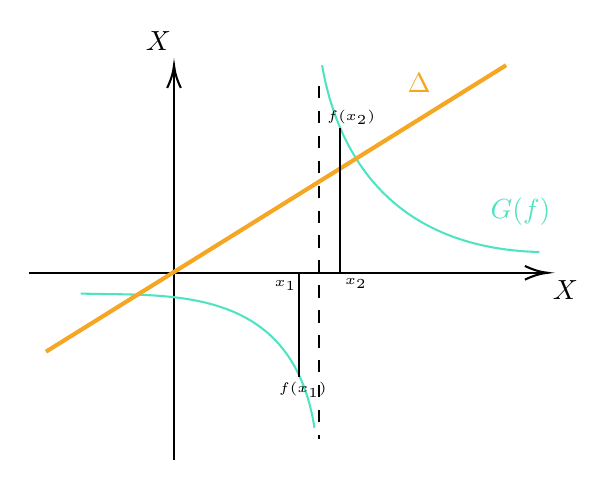
\begin{tikzpicture}[x=0.75pt,y=0.75pt,yscale=-1,xscale=1]
		%uncomment if require: \path (0,300); %set diagram left start at 0, and has height of 300
		
		%Straight Lines [id:da19790917179960688] 
		\draw    (180,140) -- (428,140) ;
		\draw [shift={(430,140)}, rotate = 180] [color={rgb, 255:red, 0; green, 0; blue, 0 }  ][line width=0.75]    (10.93,-3.29) .. controls (6.95,-1.4) and (3.31,-0.3) .. (0,0) .. controls (3.31,0.3) and (6.95,1.4) .. (10.93,3.29)   ;
		%Straight Lines [id:da6463205087944646] 
		\draw    (250,230) -- (250,42) ;
		\draw [shift={(250,40)}, rotate = 90] [color={rgb, 255:red, 0; green, 0; blue, 0 }  ][line width=0.75]    (10.93,-3.29) .. controls (6.95,-1.4) and (3.31,-0.3) .. (0,0) .. controls (3.31,0.3) and (6.95,1.4) .. (10.93,3.29)   ;
		%Straight Lines [id:da7329652606719634] 
		\draw  [dash pattern={on 4.5pt off 4.5pt}]  (320,50) -- (320,220) ;
		%Curve Lines [id:da792914158474481] 
		\draw [color={rgb, 255:red, 80; green, 227; blue, 194 }  ,draw opacity=1 ]   (321.33,40) .. controls (328.33,80.33) and (352.67,128) .. (426,130) ;
		%Curve Lines [id:da5357944547931757] 
		\draw [color={rgb, 255:red, 80; green, 227; blue, 194 }  ,draw opacity=1 ]   (317.67,214.67) .. controls (306.67,144.67) and (246.67,151.33) .. (205,150) ;
		%Straight Lines [id:da25095847185427966] 
		\draw [color={rgb, 255:red, 245; green, 166; blue, 35 }  ,draw opacity=1 ][line width=1.5]    (188.33,178) -- (410,40) ;
		%Straight Lines [id:da14232861437954414] 
		\draw    (310,140) -- (310,190) ;
		%Straight Lines [id:da822434531716816] 
		\draw    (330,70) -- (330,140) ;
		
		% Text Node
		\draw (431,142.4) node [anchor=north west][inner sep=0.75pt]    {$X$};
		% Text Node
		\draw (235,22.4) node [anchor=north west][inner sep=0.75pt]    {$X$};
		% Text Node
		\draw (401,102.4) node [anchor=north west][inner sep=0.75pt]  [color={rgb, 255:red, 80; green, 227; blue, 194 }  ,opacity=1 ]  {$G( f)$};
		% Text Node
		\draw (361,42.4) node [anchor=north west][inner sep=0.75pt]  [color={rgb, 255:red, 245; green, 166; blue, 35 }  ,opacity=1 ]  {$\Delta $};
		% Text Node
		\draw (297,142.4) node [anchor=north west][inner sep=0.75pt]  [font=\tiny]  {$x_{1}$};
		% Text Node
		\draw (331,141.4) node [anchor=north west][inner sep=0.75pt]  [font=\tiny]  {$x_{2}$};
		% Text Node
		\draw (322.33,60.07) node [anchor=north west][inner sep=0.75pt]  [font=\tiny]  {$f( x_{2})$};
		% Text Node
		\draw (299,191.4) node [anchor=north west][inner sep=0.75pt]  [font=\tiny]  {$f( x_{1})$};
		
		
	\end{tikzpicture}
\end{figure}
	Note that the diagram above is just a schematic representation of the idea behind the provided example to demonstrate some cases where $ \inv{g} $ is not continuous, and there is no particular meaning behind the fact that $ X\times X $ looks like the Euclidean 2 plane. The only case that this can fail is when all sets in $ X $ are bounded (see Exercise 3 page 46).
\end{solution}

\begin{observation}[Learning from a mistake]
	For the question above, after some discussions we found out that our answer is wrong. That is because, assuming the continuoity for $ f $, then $ d(f(x_1),f(x_2)) $ can not get very large, because
	$ d(f(x_1),f(x_2)) \leq M(x_1,x_2) d(x_1,x_2) $. 
\end{observation}






\subsection{Convergence of Sequences}
\begin{problem}
	Let $ X $ denote the set of all bounded piecewise continuous functions defined on $ 0\leq t\leq T $, with the sup-metric $ d_\infty $.
	\begin{enumerate}[(a)]
		\item Obviously $ C[0,T] $ is a subspace of $ X $. Let $ x_0 $ be an arbitrary point in $ C[0,T] $. Suppose that $ x_0 $ is to be approximated by piecewise constant functions is shows in Figure 3.6.1 in text book. That is
		\[ x_n(t) = x_0(j\frac{T}{n}) \ \text{for}\ j\frac{T}{n} \leq t < (j+1)\frac{T}{n} \ \text{and}\ j=0,1,\cdots,(n-1). \]
		and
		\[ x_n(T) = x_0(\frac{n-1}{n}T). \]
		Is it true that the sequence $ \set{x_n} $ converges in $ (X,d) $? If so, is it true that $ x_0 = \lim_{n\to\infty}x_n $? [Hint: Use the fact that a real-valued continuous function, defined on a bounded closed interval is uniformly continuous, compare with Exercise 13, Section 17.]
		
		\item Suppose $ x_0 $ is not restricted to the subspace $ C[0,T] $, and suppose that $ x_0 $ is approximated by function $ x_n $ as in (a). Is it true that $ x_0 \lim_{n\to\infty}x_n $?
		
		
		\item Consider a different metric on $ X $, namely the $ d_2 $ metric. Does the sequence $ (x_n) $ converges to $ x_0 $ in $ (X,d_2) $?
	\end{enumerate}
\end{problem}
\begin{solution}
	\begin{enumerate}[(a)]
		\item Since the points in $ C[0,T] $ are uniformly continuous, then for any choice of $ \epsilon>0 $ we can choose $ \delta>0 $ such that $ \abs{x-y}<\delta $ implies $ \abs{f(x)-f(y)}<\epsilon $. Let $ n = T/(\delta/2) $. So on each interval $ jT/n \leq t M (j+1)T/n $ we have 
		\[ \sup_{jT/n \leq t M (j+1)T/n} \abs{x_n(t) - x_0(jT/n)} < \epsilon. \]
		This also implies
		\[  \sup_{0\leq t\leq T} \abs{x_n(t) - x_0(jT/n)} < \epsilon. \]
		Thus $ x_n \to x_0 $ in $ d_\infty $ metric.
		
		\item No. The uniform continuity is crucial as observed above. For instance, consider the function $ x_0(t) = 0 $ when $ t\in [0,T) $ and $ x_0(t) = 1 $ when $ t=1 $. With the approximation scheme as above, $ x_n \equiv 0 $ for all values of $ n\in \N $, however, $ d_\infty (x_n,x_0) = 1 $ for all $ n\in \N $.`
		
		\item Yes. On any closed interval that misses one of the points of discontinuity, the function $ x_0 $ is uniformly continuous, hence on this interval $ x_n $ converges to $ x_0 $ uniformly (in sup norm), thus in $ d_2 $ norm. On the intervals that contains a point of discontinuity, we can bound the $ L_2 $ norm as follows. Choose $ n $ large enough that each point of discontinuity sits inside one interval $ jT/n \leq t < (j+1)T/n $, and the length of each interval is less than $ \eta $. Let $ \norm{x_0}_\infty = M $ and let $ K\in \N $ denote the number of discontinuities. So on the intervals that we have a discontinuity point we have
		\[ \int_{\text{on inter. w. dis. cont.}} \abs{x(t)-x_0(t)}^2 \leq M^2 K \eta, \]
		that goes zero as $ \eta\to 0 $.
	\end{enumerate}
\end{solution}

\begin{problem}
	Suppose that in a metric space $ (X,d) $ a sequence $ \set{x_n} $ converges to a point $ x_0 $. Does it follow that
	\[ d(x_1,x_0) \geq d(x_2,x_0) \geq d(x_3,x_0) \geq \cdots \geq d(x_n,x_0) \geq \cdots ? \]
	Either prove that it does, or give a counterexample.
\end{problem}
\begin{solution}
	No it does not. For instance consider the sequence $ \set{\sin(n)} $.
\end{solution}
\begin{remark}
	However in the question above, we can say if $ x_n\to x_0 $ as $ n\to\infty $, then there exists a subsequence $ \set{x_{n_k}} $ such that
	\[ d(x_{k_1},x_0) \geq d(x_{k_2},x_0) \geq d(x_{k_3},x_0) \geq \cdots   \]
\end{remark}


\begin{problem}
	Consider the metric space $ (X,d) $ given in Example 16, Section 3. Characterize the collection of all convergent sequences in $ (X,d) $
\end{problem}

\begin{solution}
	In this space a sequence is convergent if and only if it is eventually constant. Then it converges to that constant value.
\end{solution}


\begin{problem}
	Consider the sequence $ (x_n) $, where 
	\[ x_n(t) = (\cos(n!\pi t))^{2n}, \quad n=1,2,\cdots. \]
	In the metric space $ C[0,1] $ with the sup-metric $ d_\infty $. Is $ (x_n) $ a convergent sequence?
\end{problem}
\begin{solution}
	Let $ p\in \Q\cap[0,1] $ be a rational number. Then we can write $ p = \frac{a}{b} $ for $ a,b\in \N $, were $ (a,b)=1 $. We claim $ \forall n>b $ we have $ x_n(p) = 1 $. That is because
	\[ x_n(p) = (\cos(n!\pi \frac{a}{b}))^{2n} = (\cos(n(n-1)(n-1)\cdots(b!)\pi\frac{a}{b}) )^{2n}= (\cos(2k\pi))^{2n} = 1,  \]
	where $ k\in \Z $. On the other hand, for $ q\in [0,1]\backslash\Q $, since the $ \cos $ function is equal to one if and only if its argument is a multiple of $ \pi $, then $ \cos(n!\pi q) \neq 1 $ for all $ n\in \N $. So
	\[ x_n(q) = (\cos(n!\pi q))^{2n} \to 0 \quad \text{as } n\to\infty. \]
	So the limiting function $ x $ can be written as
	\[ x(t) = \begin{cases}
		1 \quad  t\in \Q\cap[0,1] \\
		0 \quad  t\in [0,1]\backslash\Q
	\end{cases}. \]
	However, $ x \notin C[0,1] $ so the sequence does not converge.
\end{solution}



\begin{problem}
	If $ \set{x_n} $ and $ \set{y_n} $ are convergent sequences in metric space $ (X,d) $, show that the sequence of real number $ \set{d(x_n,y_n)} $ converges to $ d(x_0,y_0) $ where $ x_0=\lim_{n\to\infty}x_n $ and $ y_0 = \lim_{n\to\infty}y_n $. (This exercise should be reconsidered after studying Section 7).
\end{problem}


\begin{solution}
	By the definition of converges $ x_n\to x_0 $ as $ n\to\infty $ is equivalent to $ d(x_n,x_0) \to 0 $ as $ n\to\infty $. Similarly for $ \set{y_n} $ we have $ d(y_n,y_0) \to \infty $ as $ n\to\infty $.  So using the triangle inequality for the metric function we can write
	\[ d(x_n,y_n) \leq d(x_n,x_0) + d(y_n,x_0) \leq d(x_n,x_0) + d(y_n,y_0) + d(x_0,y_0), \]
	and also
	\[ d(x_0,y_0) \leq d(x_n,x_0)+d(x_n,y_0) \leq d(x_n,x_0) + d(x_n,y_n) + d(y_n,y_0). \]
	For any given $ \epsilon>0 $ we can choose $ n $ large enough such that
	\[ d(x_n,x_0) < \epsilon/2, \quad\text{and}\quad d(y_n,y_0)<\epsilon/2. \]
	So combining the inequalities above we will get
	\[ d(x_0,y_0) - \epsilon \leq d(x_n,y_n) \leq d(x_0,y_0) + \epsilon. \]
	Or equivalently
	\[ \abs{d(x_n,y_n) - d(x_0,y_0)} <\epsilon. \]
	So $ d(x_n,y_n) \to d(x_0,y_0) $ as $ n\to\infty $.
\end{solution}


\begin{problem}
	Let $ a $ be a real number satisfying $ 0\leq a\leq 1 $ and set $ b=1-a $. Let $ y_0 =0 $ and
	\[ y_{n+1} = \frac{1}{2}(b+y_n^2). \]
	\begin{enumerate}[(a)]
		\item Show that the sequence $ \set{y_n} $ is bounded and monotone, and therefore converges. Let $ y=\lim y_n $, and $ x = 1-y $. Show that $ x^2=a $.
		\item Modify part (a) for the case $ a>1 $.
\end{enumerate}

	
\end{problem}

\begin{solution}
	\begin{enumerate}[(a)]
		\item First we show the sequence being bounded. We do it by proof by induction. First, observe that $ y_0  = 0 \leq1 $. Then assume $ y_k \leq 1 $ and we show that $ y_{k+1} \leq 1 $. This is true because
		\[ y_{k+1} = \frac{1}{2} (b+y_k^2) \leq \frac{1}{2} (1+1) = 1. \]
		So by induction $ y_n \leq 1 $ for all $ n\in \N $.
		
		To show that the sequence is monotonically increasing, we also use the proof by induction. Since $ y_0 = 0 $, we have $ y_1 = b/2 $. So $ y_1 - y_0 = b/2 \geq 0 $. Now assume $ y_{k} - y_{k+1} \geq 0 $. We want to show $ y_{k+1} - y_k \geq 0 $. Observe that
		\[ y_{k+1}-y_k = \frac{1}{2}(b+y_k^2) - \frac{1}{2}(b+y_{k-1}^2) = \frac{1}{2}(y_{k}-y_{k-1})(y_k+y_{k+1}) \geq 0.\]
		So by induction $ y_{n+1} - y_n \geq 0 $ for all $ n\in \N $. 
		
		Since $ \set{y_n} $ is increasing and bounded, then it converges. So taking the limit from both sides we will have
		\[ y = \frac{1}{2}(b+y^2). \]
		By completing the square, we will have $ (y-1) = \sqrt{1-b} = \sqrt{a} $. So $ x = y - 1 = \sqrt{a} $.
		
		\item If $ a >1 $ then we can use the following identity.
		\[ \sqrt{a} = \frac{1}{\sqrt{\frac{1}{a}}} \]
		In other words, we calculate the square root for $ a'=1/a \leq 1 $ and then we have $ \sqrt{a} = 1/\sqrt{a'} $.
	\end{enumerate}
	
\end{solution}


\begin{problem}
	Let $ \set{x_n} $ be a sequence in a metric space $ (X,d) $ with the property that for some $ \epsilon>0 $ one has $ d(x_n,x_m) \geq \epsilon $ for all $ n,m $. Show that $ \set{x_n} $ is not convergent.
\end{problem}
\begin{solution}
	Assume otherwise. So $ \exists x_0 \in X $ such that for all $ \epsilon>0 $, exists $ N\in \N $ such that $ \forall n>N $ we have $ d(x_n,x_0)<\epsilon $. This contradicts the assumption.
\end{solution}





\begin{problem}
	Let $ X = \R^n $ be given with the metric $ d(x,y) = \sum_{i=1}^n\abs{x_i - y_i} $. Show that a sequence $ \set{x_n} $ in $ X $ converges to $ x_0 $ if and only if  $ x_{n,i}\to x_{0,i} $ for all $ i=1,\cdots,n $.
\end{problem}

\begin{solution}
	\begin{enumerate}[(a)]
		\item [$ \boxed{\Rightarrow}$] Assume $ x_n\to x_0 $. Then $ d(x_n,x_0) \to 0 $. So 
		\[ \sum_{i=1}^{N} \abs{x_{n,i} - x_{0,i}} \to 0. \]
		So each term in the sum should go to zero, i.e. $ \abs{x_{n,i}-x_{0,i}}\to 0 $ as $ n\to\infty $. So $ x_{n,i}\to x_{0,i} $ as $ n\to\infty $.
		
		\item [$\boxed{\Leftarrow}$] Assume $ x_{n,i}\to x_{0,i} $ for all $ i=1,\cdots, n $. So by definition $ \abs{x_{n,i}-x_{0,i}}\to 0 $ as $ n\to\infty $. So $ \sum_{i=1}^{N}\abs{x_{n,i}-x_{0,i}} \to 0 $ as $ n\to\infty $. So $ x \to x_0 $ in $ (\R^N, d) $.
	\end{enumerate}
\end{solution}


\begin{problem}
	Let $ x_n(t) $ be a sequence of continuous real-valued functions where $ x_n(t) $ is periodic with period $ \tau_n >0 $. Assume that $ x_n(t) \to x(t) $ uniformly for $ \tau\in \R $ and $ \tau_n\to\tau $. Show that $ x(t) $ is periodic in $ t $ with period $ \tau $. 
\end{problem}
\begin{solution}
	First, observe that $ x_n(t+\tau_n) \to x(t+\tau) $ as $ n\to\infty $. Indeed, since $ t+\tau_n\to t+\tau $ as $ n\to\infty $, for any $ k\in \N $ we have $ x_k(t+\tau_n) \to x_k(t+\tau) $ that follows from continuity of $ x_n $. Because of the uniform convergence of $ x_n $, we can write $ x_n(t+\tau_n)\to x(t+\tau) $ as $ n\to\infty $. On the other hand, we want to show $ x_n(t+\tau_n) \to x(t) $. To see this 
	\[ \abs{x_n(t+\tau_n) - x(t)} = \abs{x_n(t)-x(t)} \to 0 \quad \text{as} \quad n\to\infty. \]
	So $ x_n(t+\tau_n)\to x(t) $ and $ x_n(t+\tau_n)\to x(t+\tau) $ both uniformly. Then it follows that $ x(t) = x(t+\tau) $.
\end{solution}


\begin{problem}
	Let $ f $ and $ g $ be functions in $ C[0,T] $. Define $ x_0 = f $ and $ x_1 = g $. Let
	\[ x_{n+1} = \frac{1}{2}(x_n+x_{n-1}), \quad n = 1,2,\cdots. \]
	Show that $ \lim x_n = \frac{1}{3}(f+2g) $ when $ C[0,T] $ has the sup-metric.
\end{problem}

\begin{solution}
	Let $ t \in [0,T] $. Define $ a_0 = f(t) $ and $ a_1 = g(t) $, and define $ a_n = x_n(t) $. Then $ \set{a_n} $ is a sequence of real numbers where
	\[ a_{n+1} = \frac{1}{2}(a_n + a_{n-1}). \]
	We can writ this recursive equation as
	\[ \vectt{a_{n}}{a_{n+1}} = \matt{0}{1}{1/2}{1/2}\vectt{a_{n-1}}{a_n}. \]
	So we will have
	\[ \vectt{a_n}{a_{n+1}} = A^n\vectt{a_0}{a_1}. \]
	Writing $ A $ in its Jordan block form we will have
	\[ A = P \matt{-1}{0}{0}{2} \inv{P}, \]
	where 
	\[ P = \matt{-2}{1}{1}{1}, \qquad \inv{P} = \frac{1}{3}\matt{-1}{1}{1}{2}. \]
	So 
	\[ \lim A^n = \frac{1}{3}\matt{1}{2}{1}{2}. \]
	Then it follows that $ \lim a_n = 1/3(f+2g). $ So the sequence $ \set{x_n} $ converges to the function $ h = \frac{1}{3}(f+2g) $ point-wise. To show the uniform convergence, i.e. the converges with the sup norm, we use the fact that the point-wise convergence of the uniform /.
\end{solution}


